\documentclass{article}
\usepackage{fullpage}
\usepackage{amsmath}
\usepackage{graphicx}

\title{ APC 524 Homework 4 \\
        Parallel Programming}
\author{Evan Leister}
\date {11/19/12}

\begin{document}

\maketitle

  \section{Problem Statement}

  Consider the heat diffusion equation: 

  \begin{equation}
    \frac{\partial T}{ \partial T} = \kappa \nabla^2 T
  \end{equation}

  on a domain $ 0 \leq x,y \leq \pi$ with the following boundary conditions:

  \begin{equation}
    \centering
    \begin{aligned}
      T(x,0) = \cos^2 x \\
      T(x,\pi) = \sin^2 x \\
      T(0,y) = T(\pi,y)
    \end{aligned}
  \end{equation}

  This equation can be solved as an initial value problem with an explicit timestepping scheme:

  \begin{equation}
    T_{i,j}^{n+1} = T_{i,j}^n + \Delta t \, \kappa \left( \frac{T_{i-1,j}^n + T_{i+1,j}^n + T_{i,j-1}^n + T_{i,i+j}^n - 4 T_{i,j}^n}{\Delta x ^2  }\right)
  \end{equation}

  If the end time desired is $t = 0.5 \, \pi^2 / \kappa$ and  if the grid spacing is equally spaced, the following timestep criterion applies:

  \begin{equation}
    \Delta t < \frac{\Delta x^2}{4 \kappa} 
  \end{equation}

  The above system was solved using three different implementations. 
  One implementation was a simple initial value problem where all values were calculated in serial.
  A second implementation involved programming in OpenMP in order to parallelize some of the work.
  A third implementation used OpenMPI in order to pursue a different parallelization. 

  \clearpage
  \section{Results}

  Each of these solutions took the form of figure \ref{contour}:

  \begin{figure}[ht]
    \centering
    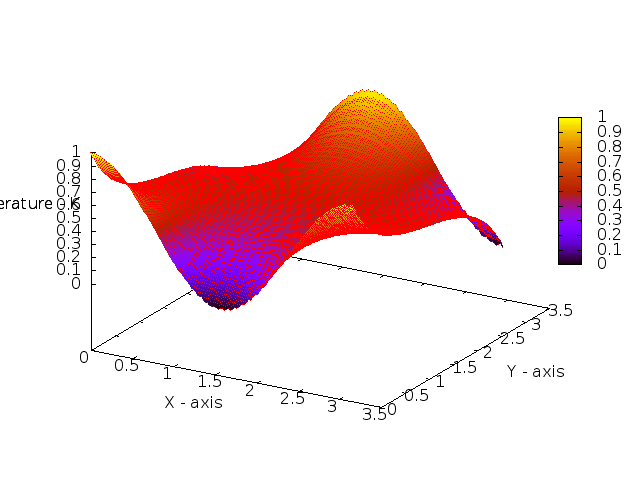
\includegraphics[scale=0.6]{128heat.png}
    \caption{ Contour plot of temperature} \label{contour}
  \end{figure}

  Each solution had an average temperature of $0.497$.

  \clearpage

  These solutions were profiled using increasing amounts of grid cells on the Adroit computing cluster. The results are collated in table \ref{adroit}.

  \begin{table}[ht]
    \centering
    \begin{tabular}{|l|l|l|l|}
      \hline
        Run Type       & 128 & 256 & 512  \\ \hline
        Serial         & 7   & 128 & 3006 \\ 
        OMP: 1 thread  & 7   & 128 & 3440 \\ 
        OMP: 2 threads & 4   & 64  & 1889 \\ 
        OMP 4 Threads  & 2   & 33  & 754  \\ 
        OMP 8 threads  & 1   & 17  & 363  \\
        \hline
    \end{tabular}
    \caption { Adroit runs, time in seconds.}\label{adroit}
  \end{table}
    
  These results were not completed due to time and queue restrictions. 
  The results in table \ref{fedora} were computed on a 4-core Lenovo i7 with simulated hyperthreading. 
  These results with 8 threads are not representative of what could be possible on a larger cluster with more processors. 
    Note that the MPI implementation was completed later than was possible to implement a complete profile test. 

  \begin{table}[hb]
    \centering
    \begin{tabular}{|l|l|l|l|l|}
      \hline
        Run Type      & 128 & 256 & 512 & 1024 \\ \hline
        Serial        & 2   & 20  & 338 & 5600 \\ 
        OMP 1 thread  & 1   & 21  & 352 & 5943 \\ 
        OMP 2 threads & 1   & 11  & 186 & 3270 \\ 
        OMP 4 threads & 0   & 7   & 100 & 3171 \\ 
        OMP 8 threads & 1   & 7   & 137 & 3296 \\
        MPI 1 threads & 1   & 18  & ~   & ~    \\
        MPI 2 threads & 1   & 11  & ~   & ~    \\
        MPI 4 threads & 1   & 6   & ~   & ~    \\  
      \hline
    \end{tabular}
      \caption{ Intel i7 runs, time in seconds} \label{fedora}
    \end{table}

    One immediate advantage of OpenMP is how simple it is to implement. 
    Obtaining a factor of two speed gain with a small piece of parallelization is not insignificant. 
    In contrast, MPI did not perform much better with slice decomposition but required a significant amount of extra programming. 
    For this problem, MPI has potential to be much faster if a more intelligent domain decomposition were used. 
    As was discussed in lecture, a square domain decomposition has a much smaller buffer for passing messages in between processes. 
    The large buffer size significantly limited the speed and reliability of larger runs. 
    
    
\end{document}
